\documentclass[pdf, hyperref={unicode}, aspectratio=169]{beamer}

\usepackage{styles}

\useoutertheme{miniframes}

\graphicspath{ {../img/} }

\title{Создание модуля управления временными рядами сигналов для системы активного мониторинга сложных технических систем}
\subtitle{Выпускная квалификационная работы бакалавра}

\pdfstringdefDisableCommands{
\def\\{}
\def\,{}
\def\textbf#1{<#1>}
}

\author[Инютин Максим Андреевич]
{
	\textbf{Студент группы М8О-407Б-19:} Инютин Максим Андреевич\\
	\textbf{Научный руководитель:} д.ф.-м.н. проф. каф. 806 Д.\,В.\,Дзюба
}

\institute[Московский авиационный институт]
{
	Московский авиационный институт (национальный исследовательский университет)\\
	Институт № 8 «Компьютерные науки и прикладная математика»\\
	Кафедра № 806 «Вычислительная математика и программирование» 
}

\date{Москва --- \the\year}

\logo{
\includegraphics[height=1cm]{mai.eps}}

\begin{document}

\epstopdfsetup{outdir=./}

{
	% убирает номер слайда с титульного слайда
	\setbeamertemplate{page number in head/foot}{}
	\frame{\titlepage}
}


\section{Актуальность темы}
\begin{frame}
	\frametitle{Актуальность темы}
	\begin{itemize}
		\item Актуальность темы данной работы связана с распространением цифровых двойников объектов и систем. Их создание позволяет моделировать отдельные процессы или объекты целиком, проводить тесты, анализировать полученные данные для подбора оптимальных параметров системы.
		\item Один из способов создания цифрового двойника --- установка сенсоров и сбор данных с них. Полученную информацию необходимо систематизировать и хранить.
		\item На предприятии может быть очень много оборудования, поэтому нужно внедрять эффективный и надёжный модуль хранения данных датчиков.
		\item Одной из актуальных областей применения цифровых двойников является создание системы мониторинга и предиктивной аналитики работоспособности газотурбинного оборудования электростанций.
	\end{itemize}
\end{frame}


\section{Цель и задача работы}
\begin{frame}
	\frametitle{Цель и задача работы}
	
	\textbf{Цель} --- разработать модуль, обеспечивающий управление структурой хранения временных рядов и данными сенсоров для системы мониторинга цифрового двойника промышленных электростанций, использующих газотурбинное оборудование.
\end{frame}


\begin{frame}
	\frametitle{Цель и задача работы}
	
	\textbf{Задачи:}
	\begin{enumerate}
		\fontsize{10pt}{12pt}\selectfont
		\item спроектировать модель данных дерева организационной структуры предприятия;
		\item описать способы взаимодействия: добавление, удаление и изменение вершин и рёбер дерева;
		\item спроектировать модель хранения временных рядов датчиков;
		\item изучить средства и технологии, которые будут применятся в ходе разработки программного продукта;
		\item реализовать модуль управления графом организационной структурой и данными;
		\item разработать алгоритм объединения данных датчиков с разными частотами дискретизации;
		\item реализовать генерацию данных для таблиц датчиков, алгоритм получения наборов временных рядов;
		\item произвести тест производительности реализованного модуля.
	\end{enumerate}
\end{frame}


\section{Постановка задачи}
\begin{frame}
	\frametitle{Постановка задачи}
	
	\textbf{Исходные данные:}
	\begin{itemize}
		\item Для работы системы мониторинга и предиктивных моделей с объектов предприятия собираются исходные данные.
		\item Оборудование оснащено датчиками, собирающими данные с разными частотами дискретезации.
		\item Так как оборудование взаимосвязано и образует сложные технологические цепочки, границы принадлежности датчика к тому или иному оборудованию размыты.
	\end{itemize}
	
	\textbf{Необходимо} разработать модуль, обеспечивающий управление структурой хранения временных рядов и данными сенсоров. Временные ряды должны хранится в ClickHouse, а справочники в PostgreSQL.
\end{frame}


\begin{frame}
	\frametitle{Постановка задачи}
	
	При реализации необходимо предусмотреть следующие особенности:
	\begin{itemize}
		\item возможность определять структуру таблиц --- наборы и типы датчиков к привязке к оргнизационной структуре;
		\item частота дискретезации датчиков может быть разной: в какой-то момент времени не у всех датчиков есть значение, тогда это событие достраивается по последнему известному значению на этот момент;
		\item датчики имеют глобальные уникальные идентификаторы;
		\item для получения данных должна быть возможность получать вектора (все значения датчиков), временной ряд, набор рядов;
		\item механизм настройки, который будет позволять сопоставлять код датчика к организационной единице;
		\item дерево оборудования связано с сигналами отношением многие ко многим.
	\end{itemize}
\end{frame}


% \section{Логика работы}
% \begin{frame}
% 	\frametitle{Логика работы}

% 	Перечислить основные разделы работы и указать их последовательность
% \end{frame}


\section{Стек технологий}
\begin{frame}
	\frametitle{Стек технологий}
	
	\begin{itemize}
		\item \textbf{Python} является основным языком программирования, который использовался при решении задач;
		\item \textbf{FastAPI} реализует веб-интерфейс для взаимодействия с модулем и базами данных, \textbf{SwaggerUI} визуализирует веб-интерфейс;
		\item \textbf{SQLAlchemy} позволяет работать с базами данных на основе объектно-ориентированного подхода;
		\item \textbf{PostgreSQL} обеспечивает хранение дерева организационной структуры предприятия и информации о датчиках;
		\item \textbf{ClickHouse} хранит большие объёмы данных, получаемые от сенсоров;
		\item \textbf{Docker} позволяет разворачивать и переносить изолированные контейнеры с базами данных;
		\item \textbf{GraphViz} визуализирует дерево организационной структуры.
	\end{itemize}
\end{frame}


\section{Архитектура решения, алгоритм решения задачи}
\begin{frame}
	\frametitle{Архитектура решения, алгоритм решения задачи}
	
	Модель графа организационный структуры:
	
	% todo Нарисовать er диаграмму (указать явно первичные и вторичные ключ)
	\begin{center}
		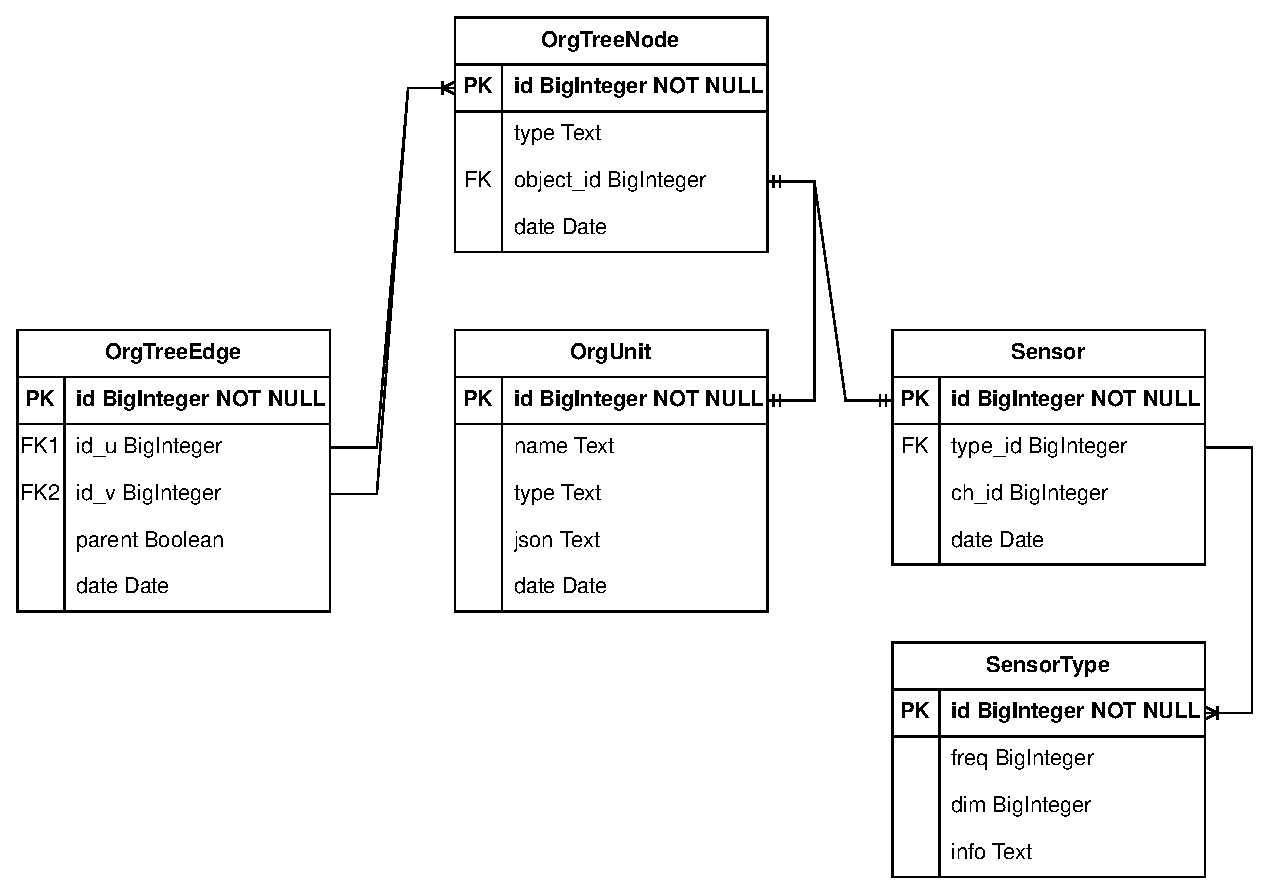
\includegraphics[height = 6cm]{pg.drawio.eps}
	\end{center}
\end{frame}


\begin{frame}
	\frametitle{Архитектура решения, алгоритм решения задачи}
	
	Основные способы управления временными рядами и деревом орг. структуры
	\begin{center}
		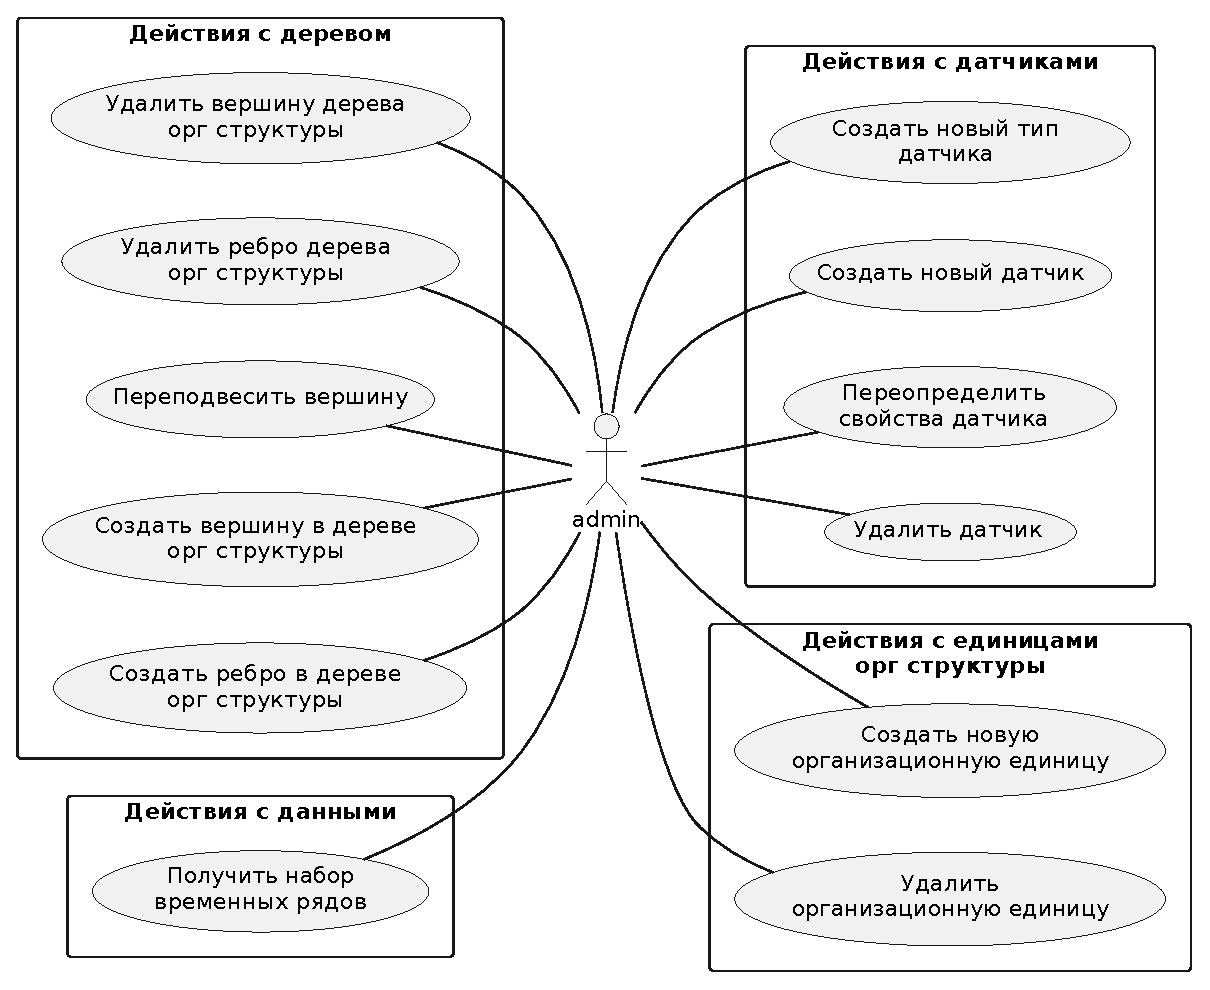
\includegraphics[height = 6cm]{usecases.eps}
	\end{center}
\end{frame}


\section{Описание программной разработки}
\begin{frame}
	\frametitle{Описание программной разработки}
	
	QR-код со ссылкой на GitHub репозиторий с исходным кодом
	
	\begin{center}
		
\includegraphics[height = 6cm]{qr-git.eps}
	\end{center}
\end{frame}


% \begin{frame}
% 	\frametitle{Работа с данными (???)}

% 	\begin{itemize}
% 		\item Обучающая выборка
% 		\item Тестовая выборка
% 		\item Источники
% 		\item …
% 	\end{itemize}
% \end{frame}


\section{Результаты разработки}
\begin{frame}
	\frametitle{Результаты разработки}
	
	Для демонстрации программного продукта используется OpenAPI SwaggerUI
	
	\begin{center}
		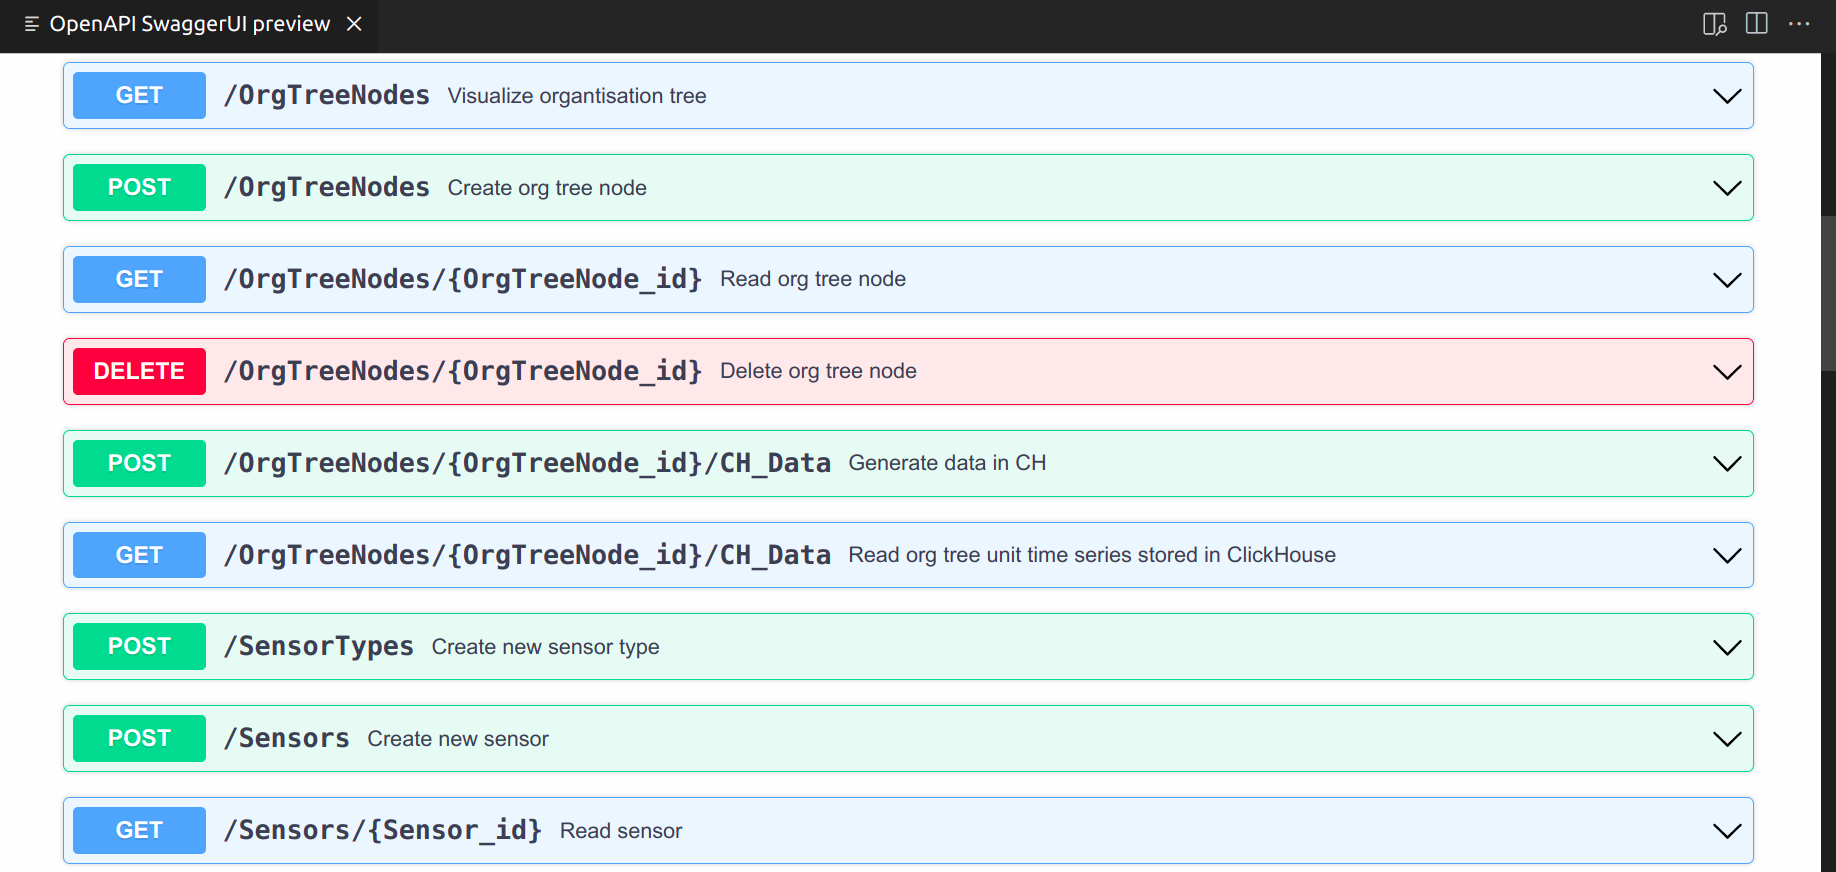
\includegraphics[height = 6cm]{swagger1.png}
	\end{center}
\end{frame}


\begin{frame}
	\frametitle{Результаты разработки}
	
	Справочная информация в SwaggerUI
	
	\begin{center}
		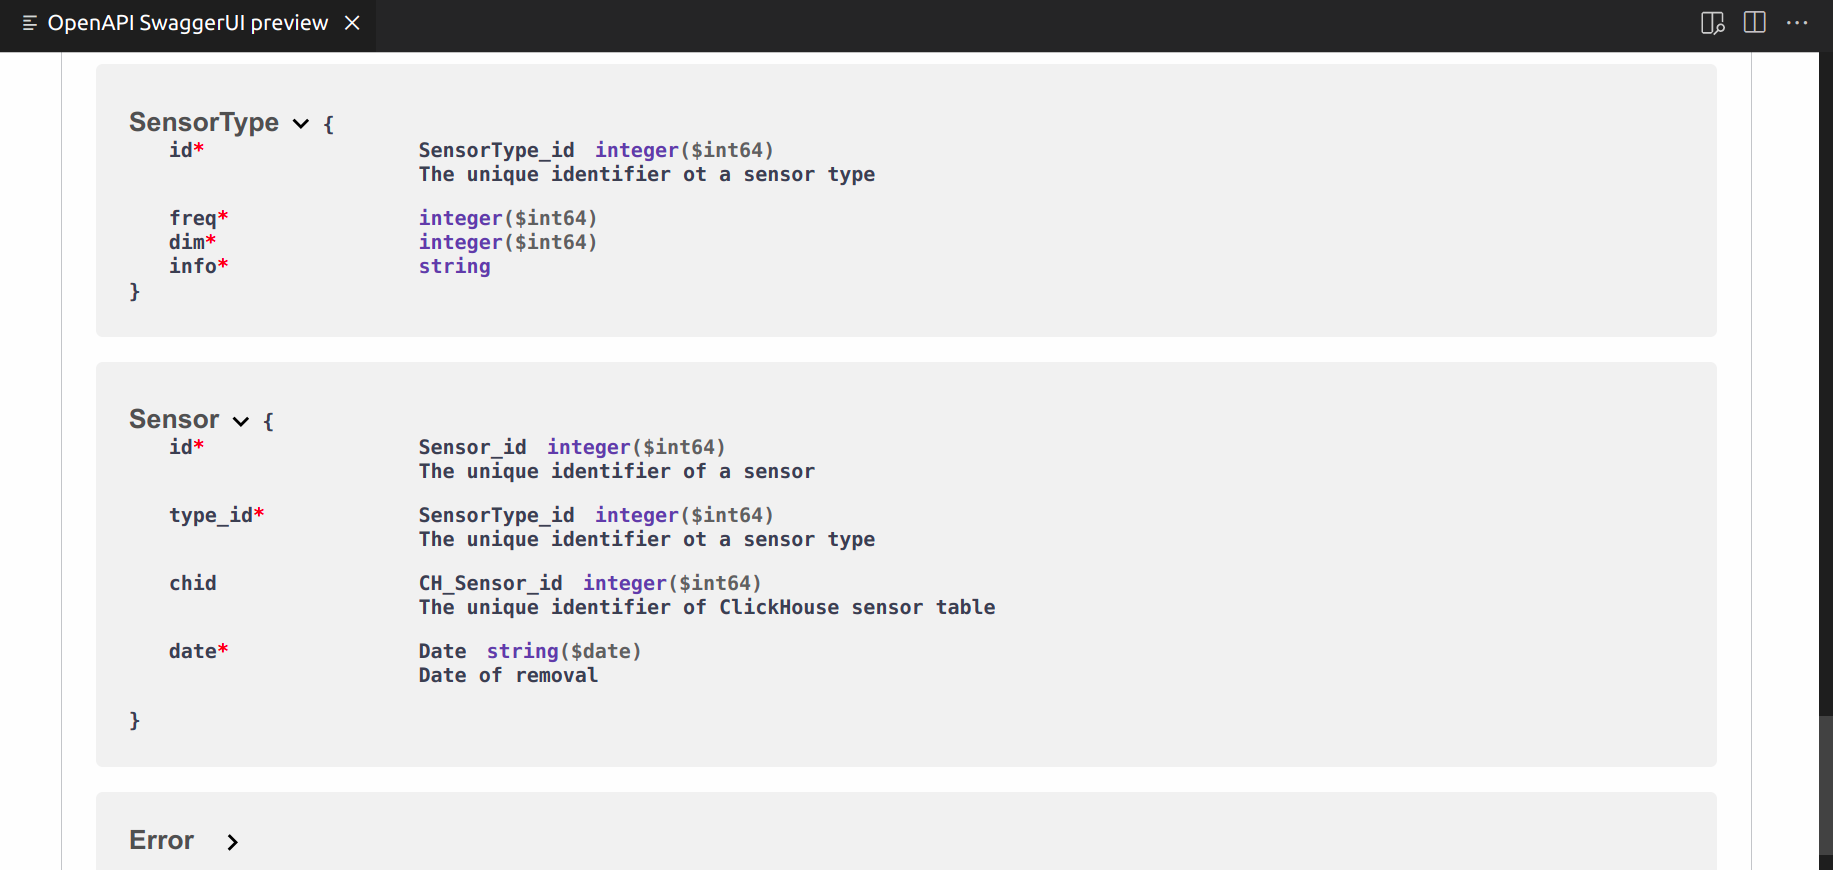
\includegraphics[height = 6cm]{swagger2.png}
	\end{center}
\end{frame}


\begin{frame}
	\frametitle{Результаты разработки}
	
	Визуализация дерева организационной структуры
	
	\begin{center}
		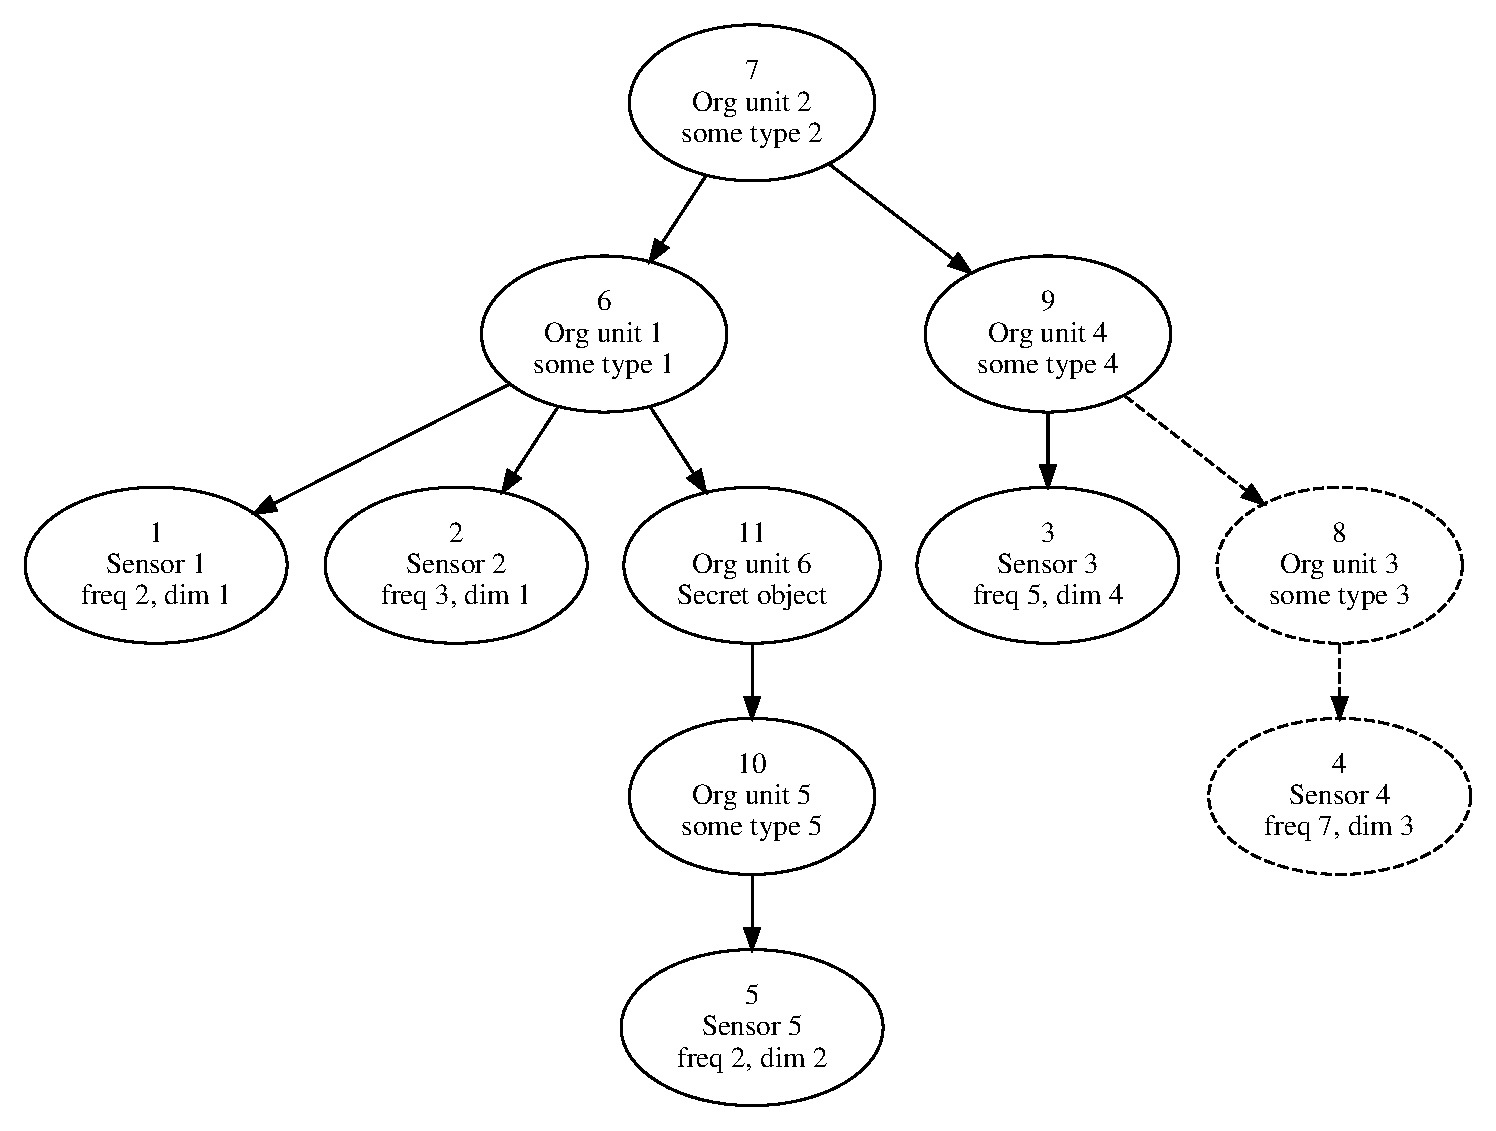
\includegraphics[height = 6cm]{demo_del8.eps}
	\end{center}
\end{frame}


\begin{frame}
	\frametitle{Результаты разработки}
	
	Получение набора временных рядов с датчиков $1$, $2$, $5$
	
	\begin{center}
		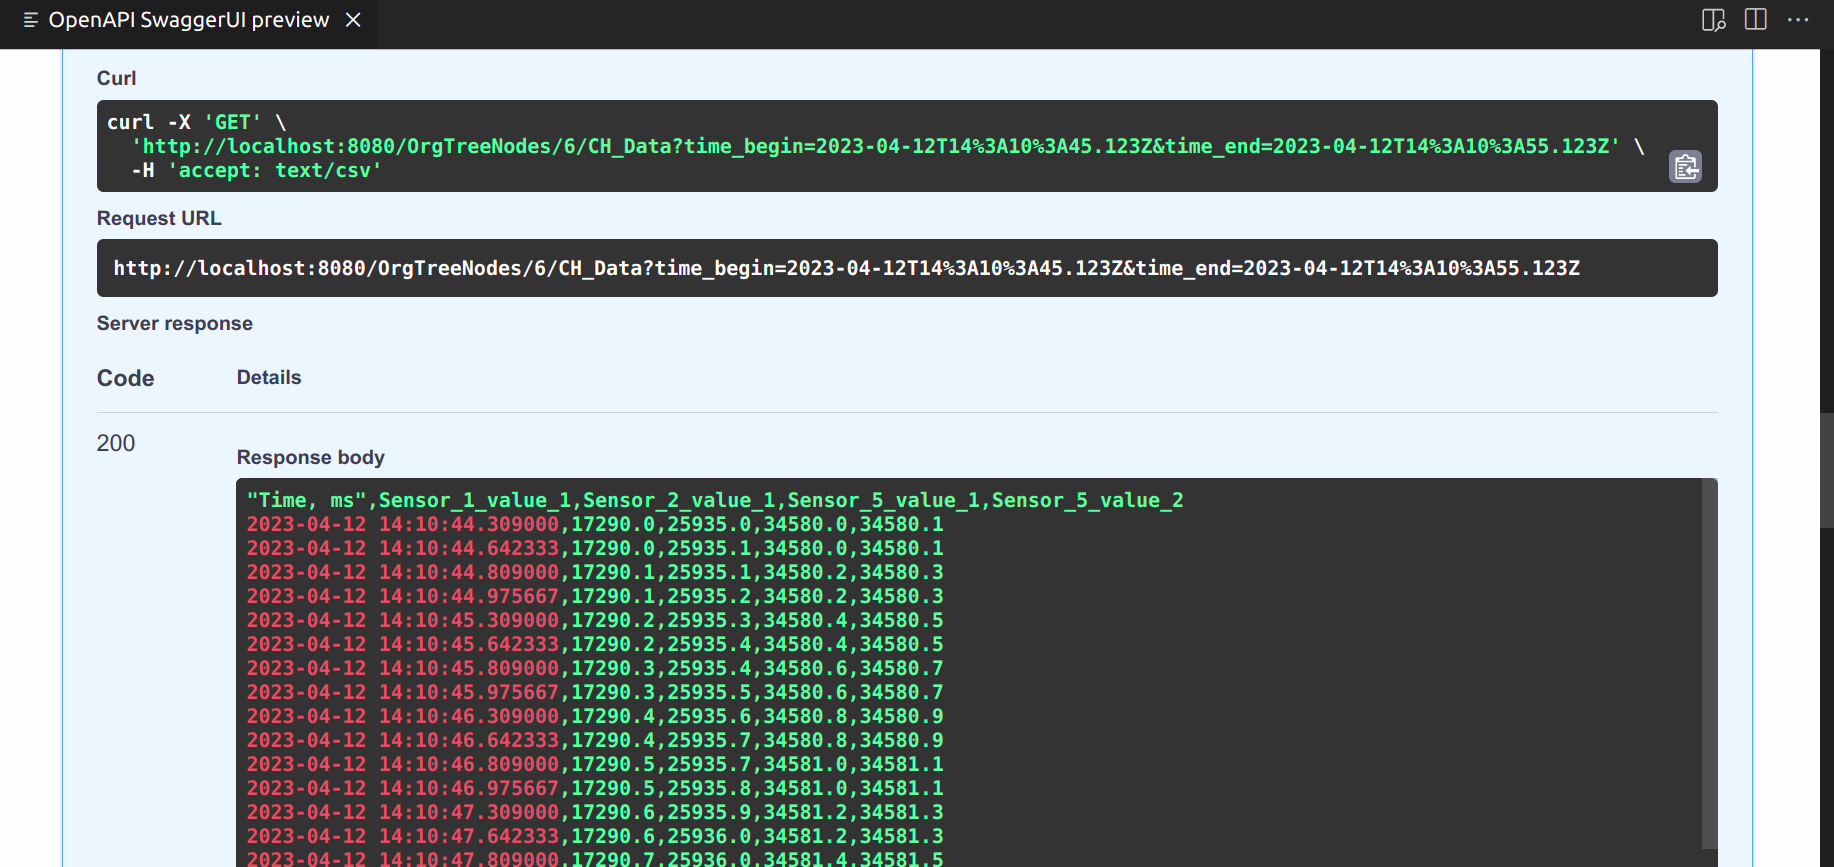
\includegraphics[height = 6cm]{swagger8.png}
	\end{center}
\end{frame}


\section{Способы хранения временных рядов}
\begin{frame}
	\frametitle{Способы хранения временных рядов}
	
	\begin{itemize}
		\item \texttt{multi} --- каждому датчику соответствует отдельная таблица в ClickHouse.
		\item \texttt{single} --- единая таблица для всех датчиков, в которой предварительно выполнена интерполяция данных.
	\end{itemize}
	
	Необходимо сравнить способы и выбрать более эффективный с точки зрения вычислительных ресурсов.
\end{frame}


\section{Тесты производительности}
\begin{frame}
	\frametitle{Тесты производительности}
	
	Графики времени обработки запроса для диапазонов до $20000$ секунд
	
	\begin{center}
		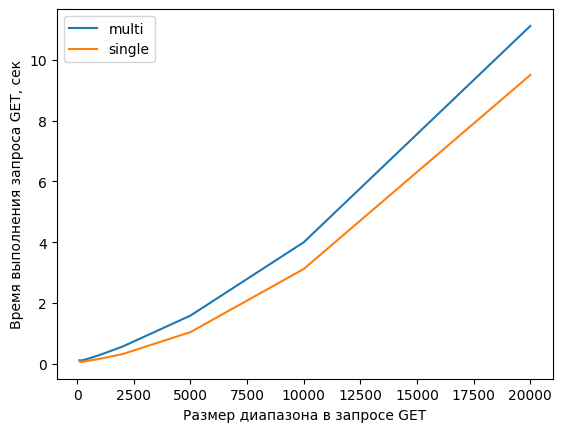
\includegraphics[height = 6cm]{bench2e4.png}
	\end{center}
\end{frame}


\begin{frame}
	\frametitle{Тесты производительности}
	
	Графики времени обработки запросов для больших диапазонов
	
	\begin{center}
		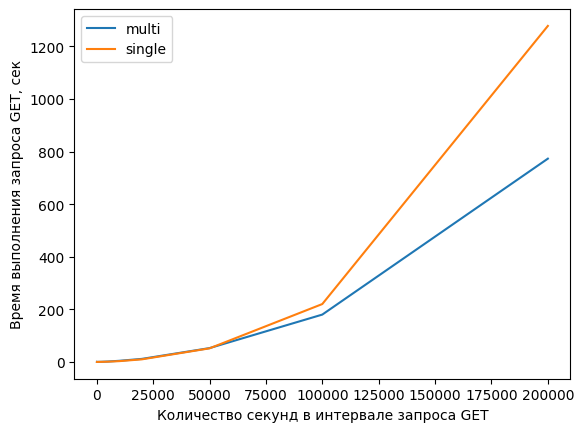
\includegraphics[height = 6cm]{bench2e5.png}
	\end{center}
\end{frame}


\section{Оценка результата}
\begin{frame}
	\frametitle{Оценка результата}
	
	\begin{itemize}
		\item В результате выполнения ВКР был разработан модуль управления временными рядами сигналов сложных технических систем на языке Python с использованием СУБД PostgreSQL и ClickHouse.
		\item Модуль автоматизирует сбор информации с сенсоров системы, тем самым упрощая создание цифрового двойника электростанции.
		\item Данные с датчиков надёжно хранятся в базе данных и будут использованы для моделирования объекта и предиктивной аналитики.
		\item Можно будет оптимизировать работу оборудования, замедляя темпы его износа, повысить отказоустойчивость как отдельной электростанции, так и всей электросети в целом.
	\end{itemize}
\end{frame}


\section{Отзывы и рецензия}
\begin{frame}
	\frametitle{Отзывы и рецензия}
	
	\begin{columns}
		\column{0.5\textwidth}
		\center{Скан отзыва научного руководителя}
		
		\column{0.5\textwidth}
		\center{Скан рецензии}
	\end{columns}
\end{frame}

\end{document}
